\section{Introduction}
The foundation for the work presented in this thesis is the lightweight robotic arm developed throughout several student projects, the latest being the semester
thesis\parencite{zeitlerDevelopmentRoboticArm} and master thesis\parencite{zeitlerDualArmAerialManipulation} of Samuel Zeitler. Over the course of these previous projects, 
a lightweight robotic arm was developed as seen in \autoref{fig:prev_robotic_arm}.

\begin{figure}
    \centering
    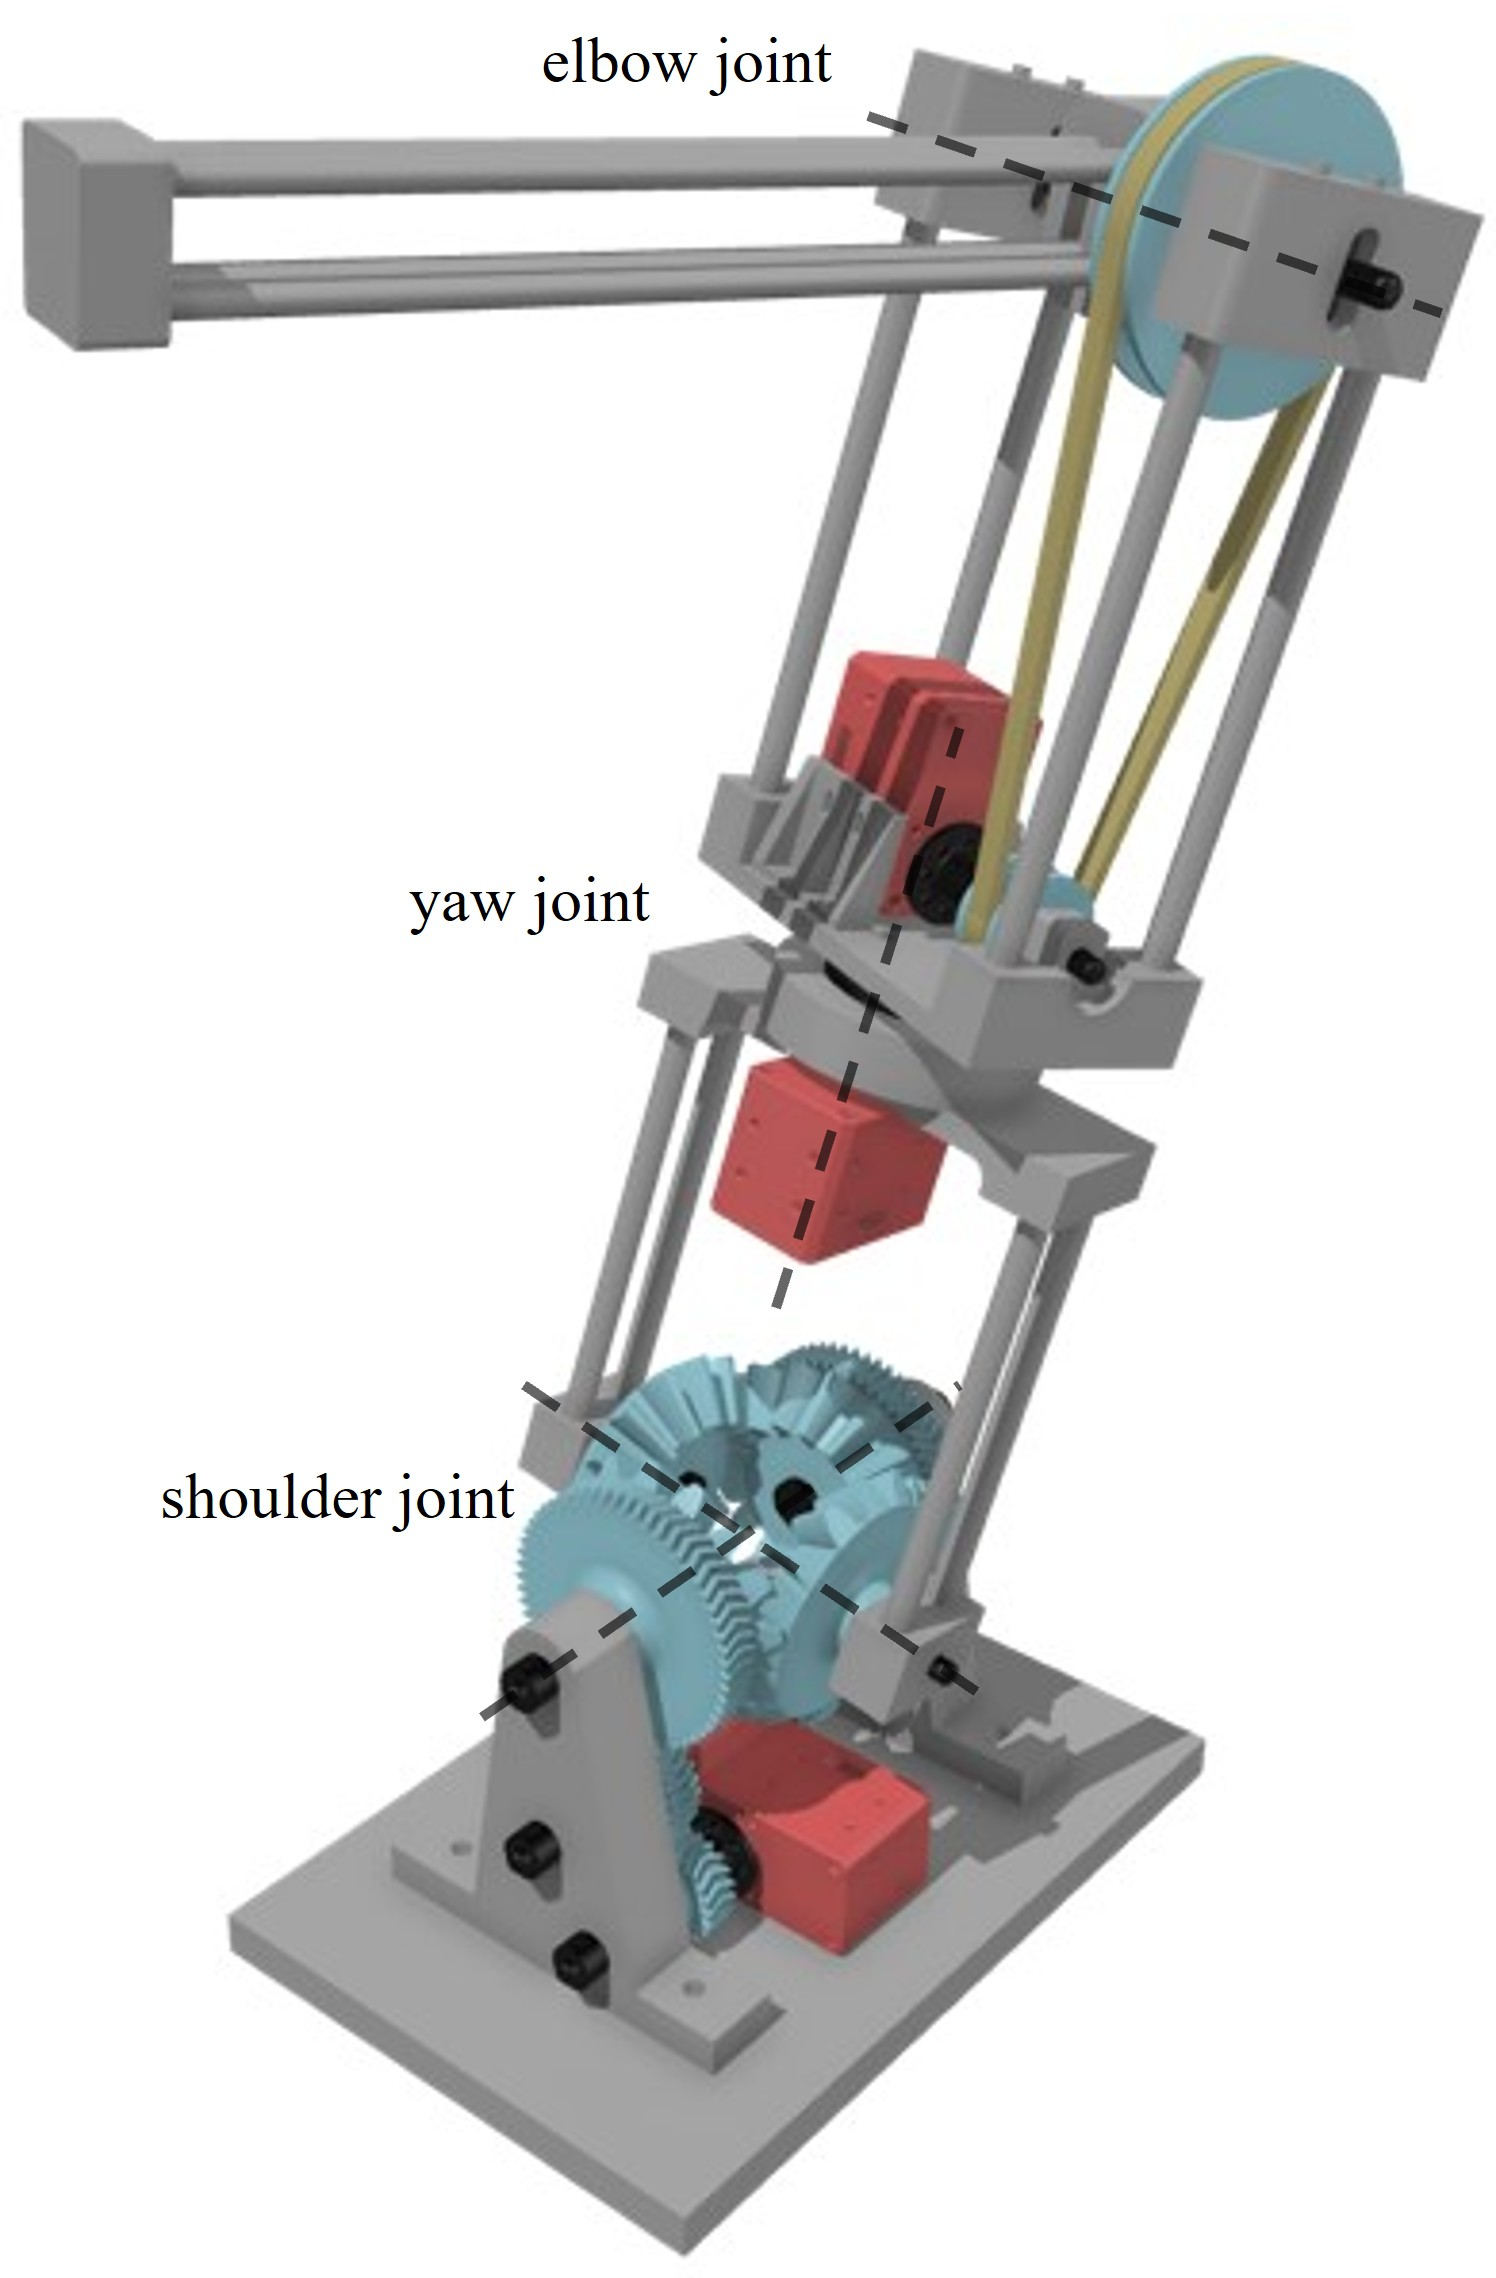
\includegraphics[width=0.8\linewidth]{images/prev_robotic_arm.jpg}
    \caption{Lightweight robotic arm prototype as designed by Samuel Zeitler}
    \label{fig:prev_robotic_arm}
\end{figure}

The robotic arm consists of several joints, resulting in four degrees of freedom in total.
The shoulder joint has two degrees of freedom, the yaw joint and elbow joint each have one.
This ensures a range of motion wide enough for the demonstration purposes.
This existing prototype was designed with the goal of mounting it on a drone, which is why the focus was on a lightweight design.
Since the robot arm is now intended to be used as an experimental platform for the exploration of robotic arm control strategies at the Chair of Automatic Control Theory,
the main focus of this thesis is to enhance the existing prototype to improve accuracy, robustness and durability.

The existing prototype is controlled using a MATLAB-based software suite, which was also developed in previous student projects. This software utilizes the servos' integrated
velocity control for a velocity-based control approach of the robotic arm. In this thesis, the current control capabilities of the servos are explored to enable torque-based 
control strategies. Specifically, the indirect torque measurement capabilities of the servos are investigated and utilized to implement basic torque reading functionality.

The following chapters will detail the enhancements made to the hardware of the robotic arm, the implementation of a basic torque reading strategy and the exploration of torque-based control.